\documentclass[a4paper,10pt]{article}
\usepackage[utf8]{inputenc}
\usepackage[left=2cm,right=2cm,top=2cm,bottom=2cm]{geometry}
\usepackage{graphicx}
\usepackage{amssymb,amsmath}
\usepackage{caption}
\usepackage{float}
\usepackage{hyperref}

%opening
\title{\textbf{Machine Learning Lab} \\ \textbf{ Miniproject 1} \\ \textbf{Apes mating calls classification}}
\author{Razvan-Andrei Stoica}
\date{\today}

\begin{document}

\maketitle

\section{Task description}
The main scope of this lab project was to classify 9 primates based on individual recordings of their mating calls. This problem falls into the category of classification tasks of machine learning. However, given the dynamic characteristics of sound waves, it is not a static classification task , but a dynamic one.  This could also be seen in the data where the sample utterances had different discretized lengths. 

\subsection*{The data}
The data provided for this classification task contained two sets: one of training, and respectively, another one of testing. The training set comprised of 270 sample with even numbers of 30 recordings per subject, while the testing set was formed of 370 recordings with varying numbers of utterances per subject. Both, the training set and the testing set had the representation $(X_i,y_i)$. $X_i$ stood for a matrix form of an utterance, with discretized frames displayed on the vertical dimension, and respectively, their corresponding features on the horizontal direction, while $y_i$ was the class label marking the mammal that produced the utterance. Hence, the classification task could be approached through via supervised learning algorithms.

The features were represented by pre-processed 12-length vectors of coefficients standing for the estimates of frequency band energies at discrete frames. Since, more data on the features was not provided, and they were detailed as being extracted via typical methods of speech signals pre-processing, they were considered as given.

\subsection*{The challenge}
This problem presented a couple of challenges worth to be mentioned. Firstly, one had to handle the different length of the utterances in training. Secondly, the discrimination against classes could not be seen at the raw level plots of the data set, which suggested that the recordings were pretty similar. Therefore, this classification problem raised the motivation to come up with a classifier able to perform the task under the given conditions.  

\section{Approach}
Given the problem, we considered each subject to be an abstract source capable of mapping the same conceptual utterance to different forms via a function $f_c(sound) = X$, with $c=1...9$. Therefore, our aim was to reproduce such functions $f_c$ in the hope of being able to recognize the mammal producing the sound by its characteristic emission function trained in supervised fashion. Therefore, we based our classifier on a feedforward neural network, which is able to reproduce in theory arbitrarily well smooth functions. Hence, our model for this classification task was feedforward neural networks.

Furthermore, we had to handle the problem of varying recording lengths. We did so following the consideration that speech utterances are short time stationary, and hence, by truncating an utterance up to its first couple of frames we would see typically the same values of the features from frame to frame. Moreover, comparing different individuals up to the same frame length from the beginning of the utterances would underline some of the discriminating differences laying in the feature values.  

Given the high level motivation, let us now present in full scope our training algorithm for the selected model on the training data set.

\paragraph{STEP1:} Having decided on a model for a classifier, we set its capacity. Therefore, we considered for this problem a 3 layer feedforward network with one hidden layer of neurons as shown in figure (\ref{fig:ffnn}). The number of units in the hidden layer was variable, and was subject to optimization through cross-validation. The activation function considered for our network was the logistic sigmoid, i.e. 
\begin{eqnarray}\label{eq:activ}
g(\vec{x}) = \frac{1.0}{1.0 + \exp({-\vec{x}})}
\end{eqnarray} applied element-wise. 

\begin{figure}[ht!]
\centering
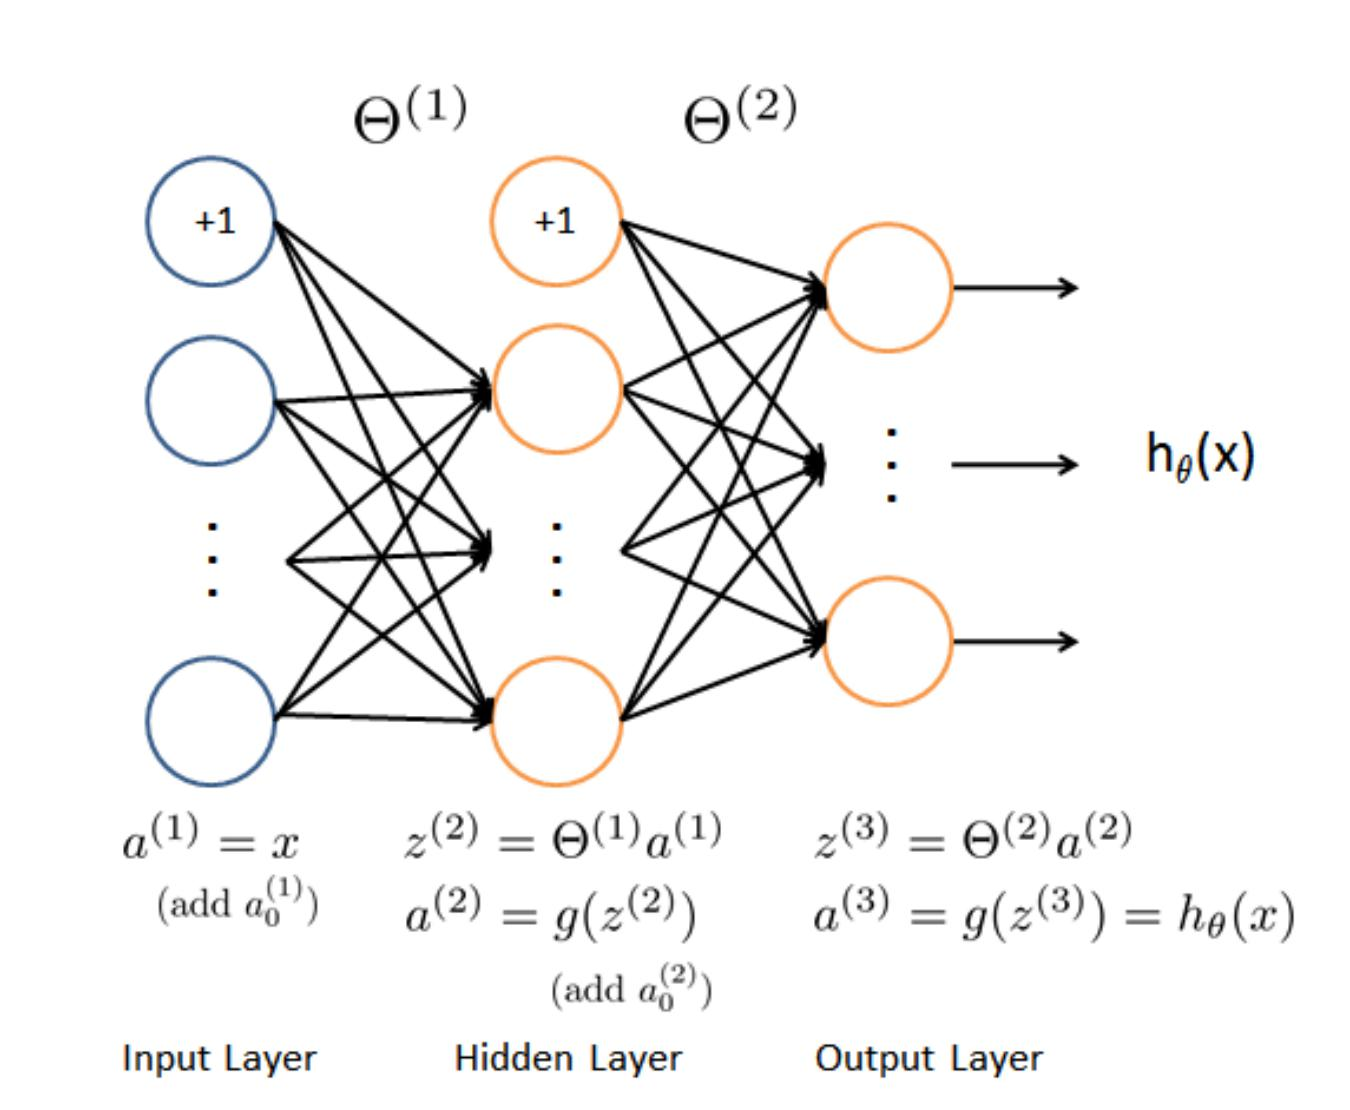
\includegraphics[scale=0.5]{ffnn}
\caption{Feedforward 3-layer neural network}\label{fig:ffnn}
\end{figure}

In figure (\ref{fig:ffnn}), $\Theta^{(i)}$ stands for the weights matrix from layer $i$ to layer $i+1$, $a^{(i)}$ represents the units activation values at layer $i$ and $h_{\Theta}(x)$ is the network output to the input $x$. 

Since we had, a 9 classes classification problem with a feature space dimension of 12, we considered the number of input units $Ni = 12$, and the number of output units $No = 9$ to be fixed. In addition, for simplified notation, the number of hidden units parameter was denoted by $Nh$. 

\paragraph{STEP2:}We iterated through the training sample points and extracted the minimum recording length $min_{rec}$ and we cropped all the utterances up to this frame. In this way, we handled the varying recordings' length while following our previous remark on this topic.

\paragraph{STEP3:}Using the random weights initialization, forward-propagation and back-propagation algorithms paired with the activation function (\ref{eq:activ}) and the logistic regression cost function, as given in \cite{an},
\begin{eqnarray}\label{eq:cost}
L(\Theta;Nh,\lambda) &=& -\frac{1}{N}\sum_{i=1}^{N}\sum_{k=1}^{K}\left[y_{i,k}\log(h_{\Theta}(x_i))_k + (1-y_{i,k})\cdot(1-\log(h_{\Theta}(x_i))_k)\right] \\\nonumber &+& \frac{\lambda}{2N}\left[\sum_{j=1}^{Nh}\sum_{j=1}^{Ni}(\Theta^{(1)}_{j,k})^2) + \sum_{j=1}^{No}\sum_{j=1}^{Nh}(\Theta^{(2)}_{j,k})^2)\right],
\end{eqnarray}
where $y_{i,k}$ stands for the the $k$-th component of the $i$-th target that the network is expected to achieve, and respectively, $(h_{\Theta}(x_i))_k$ is the $k$-th component of the $i$-th network response, corresponding to the $i$-th input $x_i$ (i.e. $h_{\Theta}(\cdot)$ denotes generically the network "response" function parameterized on the network weights $\Theta$), we trained the network weights $\Theta^{(1)}$ and $\Theta^{(2)}$. In fact, we solved the unconstrained optimization problem 
\begin{eqnarray}\label{eq:opt_pb}
\min_{\Theta} L(\Theta;Nh,\lambda),
\end{eqnarray}
where the regularization coefficient $\lambda$ is regarded as a parameter which in fact constraints the weights to stay at low values ensuring that the network does not start to overfit the data samples for high capacity models, such that the bias-variance dilemma is handled during training as well. The optimization problem was done using the conjugate gradient method.

Our choice of the network cost function was motivated by the yes / no classification type of decision that should be taken on each of the potential classes for the individual inputs to the network. Moreover, this error function couples well with the logistic sigmoid activation function.

\paragraph{STEP4:}We iterated \textbf{STEP3} over a span of parameters $Nh$ and $\lambda$ in order to perform cross-validation of the network training algorithm. Thus, we have found optimal values $Nh_{opt}$ and $\lambda_{opt}$ in the ranges considered and we used these to retrain the network weights for evaluation.

\paragraph{STEP5:}We tested the network obtained after \textbf{STEP4} on the test data set. In doing so, we considered the test inputs $(X_i,y_i)$. We removed the class pair component $y_i$ and worked on $X_i$ only. We passed the entire utterance $X_i$ to the network and performed classification on each frame. We tried therefore, to be consistent to our idea of stationary utterances with respect to close-by frames. We considered this approach thinking that a frame should sub-in for approximately 15-25 ms in time. Since we had no previous information on the pre-processing besides the one outlined in the beginning of this report, we just considered therefore the average time for such a feature extraction approach. This would thus translate for a mean average of 17 frames per utterance into 340 ms, which we considered to be enough for a mating call to be thought of as stationary. 

Consequently, passing the full utterances to the network we employed the majority rule for the classification of the recording. Thus, every frame would be classified and then the class with the most attributed frames would be the class considered for the entire recording.

\section{Implementation}
The code for this project was implemented in MATLAB, and consists of:
\begin{itemize}
\item initFFNN.m
\item randInitWeights.m
\item feedForward.m
\item costFunction.m
\item fmincg.m \cite{fmincg}
\item crossValidation.m
\item testMyClassifier.m
\item classifyApe.m
\end{itemize}

The implementation of all the aforementioned functions has been commented in the source code. Nonetheless, we will go through the training algorithm for additional clarity, since we implemented it using a third party optimization function.

\subsection{The training}
In training the network we used the following pseudo-code typical for a forward / backward gradient oriented training algorithm of a feedforward neural network.

\begin{verbatim}
randomly initialize weights
for training_sample in training_data:
    forward_propagate(training_sample)
    calculate cost_function
end
for training_sample in training_data:
    forward_propagate(training_sample)
    backward_propagate(training_sample)
    for all weights
        accumulate partial_derivatives
    end
end
roll up gradient out of partial_derivatives
regularize and normalize gradient
conjugate gradient optimization of cost_function
get optimum_weights
end
\end{verbatim}

The typical gradient descent method was replaced by the conjugate gradient optimizer in order to provide a faster and more stable solution with a better memory payload which would allow a finer cross-validation on top of the training algorithm. This was done after the gradient descent method failed to provide satisfactory results for the optimization problem in relatively short time, such that cross-validation would be possible.

The \textit{fmincg.m} function is available under a free-license, being ported to other programming languages  as a optimization procedure which finds the minimum of a function starting from an initial value given that the gradient of the function is also provided. Therefore, we first used back-propagation to compute the gradient of the cost function and then we called \textit{fmincg.m} on the cost function handle with the starting parameter values. This approach solved both problems of slowness and numerical instability we have previously encountered using the gradient descent method to find the minimum of the cost function $L(\Theta;Nh,\lambda)$.

\subsection{The cross-validation}
In our notation for the cost function, we have used as parameters $Nh$, the number of hidden units, and respectively, $\lambda$, the regularization term, while all the weights $\Theta$ were regarded as arguments to the function. Hence, we considered cross-validation for our training algorithm at the level of the $Nh$ and the $\lambda$ parameters.

\subsubsection{The partitions}
We first truncated the recordings to the frame size of the shortest which was 7 frames for recording number 69 out of the initial training inputs of 270. Hence we obtained $7*30*9 = 1890$ sample points, following our considerations for training as outlined earlier. Out of these $1890$ sample points, we have an even distribution of $210$ sample points per class, and respectively $30$ sample points of frame $0$ of each class, $30$ sample points of frame $1$ of each class, and so on, up to frame $7$. Therefore, we maintain the balance in the data between training and validation sets and consider a $7$-fold validation setup where we select for the validation step frames number $1$ over all the utterances (obtaining thus a validation set of $270$ sample points, i.e. $30$ sample points per class), then we continue with frames number $2$ over all utterances and so on until we end up again considering frames number $1$. Performing this $7$-fold partitioning and cross-validation we also model the influences different frame positions have on the validation error. 

In our cross-validation, we varied $Nh$ in $Nh = 10:2:30$, as we considered that having a 9 class classification problem we would require at least 9 units in the hidden layer to account for any possible non-linearities modeled by each individual class, and respectively, we varied $\lambda$ in $\lambda = [0,logspace(-1,1,19)]$ in order to have covered cases where the regularization was turned off, and where it was reducing the capacity of the model (for higher values of $\lambda$). As a consequence, we had a cross-validation grid of $11 \times 20 = 220$ parameter pairs.  

\subsubsection{The validation}
After having trained the network for one parameter pair, we validated the weights on the validation step using forward propagation and comparing the output of each sample point in the validation set against its known target reference. Therefore, by minimizing the misclassification error percentage for each value pair, we wanted to ensure that individual frames are classified as accurate as possible for all the classes where they belong to. In doing so, we aimed for a better classification of the full utterances in the end, as our majority rule, would act as a average or smearing out operation, which should improve the frame by frame classification by some degree. 

\subsubsection{The results}
In running the cross-validation, we stored the train and validation errors for each value pair and we plotted figure (\ref{fig:cv}). From there we observe that classifier needs to have a high capacity in order to classify  satisfactory the data, as for large values of $\lambda$ both the train and the validation errors are approaching or exceeding $30 \%$. This suggests that the discrimination boundaries between the different classes are non-linear and not simple in shape. Thus,  the network needs more hidden units in order to discriminate well among different classes. 

In addition, it is clear that the neural network operates well for small or no regularization at all, as the surface is slanted towards the $0$ regularization coefficient, where we also find the optimal result for $\lambda_{opt} = 0$.

\begin{figure}[ht!]
\centering
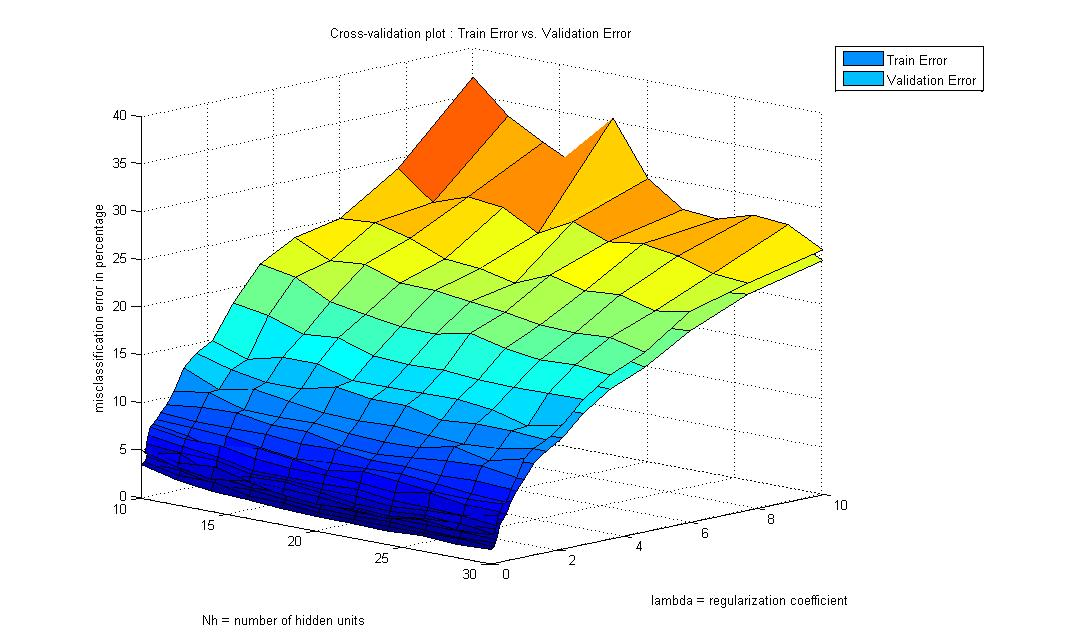
\includegraphics[scale=0.45]{cv}
\caption{Cross-validation test error vs. validation error surface plot}\label{fig:cv}
\end{figure}

Moreover, we plot the training and the validation misclassification errors for this optimal parameter value of $\lambda$ in order to see better what is happening in the case of $Nh$ (figure (\ref{fig:cv_H})). In figure (\ref{fig:cv_H}), we remark an almost constant small difference in the misclassification percentage between the train and the validation error. This behavior could also be remarked at the level of the surface plot, which justifies our initial belief that frames are short-time stationary, since also the validation data set tests well. However, we remark that as the network starts overfitting the validation error starts to oscillate, point at which we just considered the number of hidden units that rendered the best validation error so far, i.e. $Nh =24$.   

\begin{figure}[ht!]
\centering
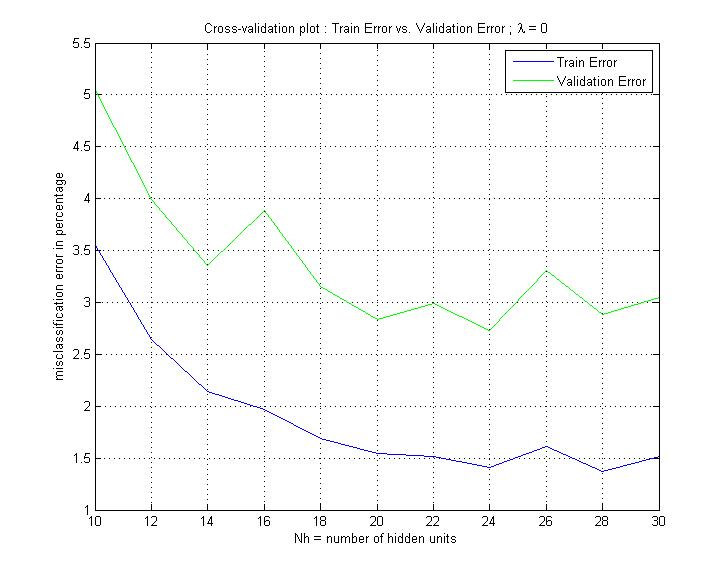
\includegraphics[scale=0.45]{cv_H}
\caption{Cross-validation test error vs. validation error plot ; $\lambda = 0$}\label{fig:cv_H}
\end{figure}

\section{Results}
After we ran the cross-validation and found the best value pair for our considered ranges, we picked the parameters $Nh_{opt} = 24$ and $\lambda_{opt} = 0$ and used them in training a new network to test our classifier design on the test data set. The network trained with these two parameters  was firstly stored in the file \textit{opt\_net.mat} for later reuse and then used in testing as described in the Approach Section. Hence, running the script \textit{testMyClassifier.m}  returned the following results:

\begin{verbatim}
Misclassification percentage on testing dataset is 5.135 %
\end{verbatim}

Nonetheless, we remark that given the random initialization of the weights, the misclassification result can slightly differ, but taking the average over 50 runs yielded an average misclassification rate of $5.647\%$.  For this reason, an auxiliary script to create neural network for scratch has been written, such that if one wishes the classifier can be generated on the spot using the optimal $Nh = 24$ and $\lambda = 0$ parameters, and then used for testing. The choice between using the stored network and generating it on the spot is documented in the \textit{trainMyClassifier.m} file.

\section{Conclusion}
The problem of pattern recognition is a problem of general interest in machine learning. Given the information enclosed by the data set it can be straightforward (as easy as separating two far apart points with a line) or complicated (as in the present case). Nonetheless, there are advanced methods which allow such problems, either in their static or dynamic representation, to be solved. 

For the present assignment, we have made use of a feedforward neural network classifier trained with the back-propagation and conjugate gradient optimization approach in order to classify a 9 class dynamic speaker recognition problem.  Here are some insights on the method we used and some potential improvements:
\begin{itemize}
\item It was advantageous to use such a design for implementing a classifier in this situation as the neural network was able to handle the data set, in the sense that it could discriminate among classes with a relatively high resemblance.

\item The network responded well to few training samples and learnt to discriminate among the recordings fast.

\item Our assumption that frames are short-time stationary combined with the truncation of recordings to the shortest one improved the training by providing extra sample points from a relatively low training data set.

\item The majority decision implemented also improved the per recording classification by averaging out misclassifications of frames.

\item The conjugate gradient method of optimization improved accuracy and speed of training when compared to the simple gradient descent.

\item The cross-validation (even on a relatively constrained grid) took a long time to run (approximatively 10 hours).

\item If means of time and hardware were to be met, it would be nice to create multiple networks and perform classification of the level one-vs-all. In this case, a higher accuracy would be expected.
\end{itemize}

\textbf{NOTE:} Some of the implementation details related to the backpropagation algorithm follow up from \cite{an}, while the underlying theory has been studied from both \cite{hj} and \cite{an}. 

All in all, the project led us to learn about feedforward neural networks, forward propagation, backpropagation, gradient descent and conjugate gradient optimization methods at a practical level.

\begin{thebibliography}{3}
\bibitem {hj} H. Jaeger, Machine Learning Lecture Notes, Jacobs University Bremen, Machine Learning Course, Fall 2011, Ch. 8, updated 29.03.2013, \href{http://minds.jacobs-university.de/sites/default/files/uploads/teaching/lectureNotes/LN_ML_Fall11.pdf}{LN\_ML\_Fall11.pdf}.
\bibitem {an} A. Ng, Machine Learning Lecture Notes, Stanford University, Coursera online course,  Lectures 8 \& 9, Fall 2014, \href{https://www.coursera.org/course/ml}{https://www.coursera.org/course/ml}.
\bibitem {fmincg} C. E. Rasmussen, Optimization solver based on conjugate gradients. Octave implementation last updated at 13.02.2002, Free License, \href{http://www.mathworks.com/matlabcentral/fileexchange/42770-logistic-regression-with-regularization-used-to-classify-hand-written-digits/content/Logistic%20Regression%20with%20regularisation/fmincg.m}{fmincg.m --- FileExchange}.
\end{thebibliography}
\end{document}
